\subsection*{1D reads}

        The following histograms show the length distribution of 1D reads (both template and complement) for passes and fails.

        \begin{tabular}{cc}
          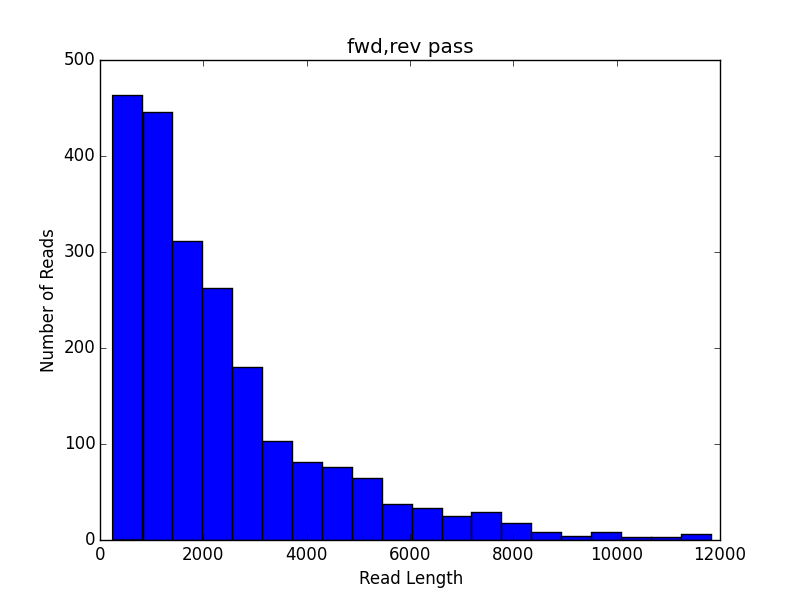
\includegraphics[width=.48\textwidth]{1Dpasses}
          &
          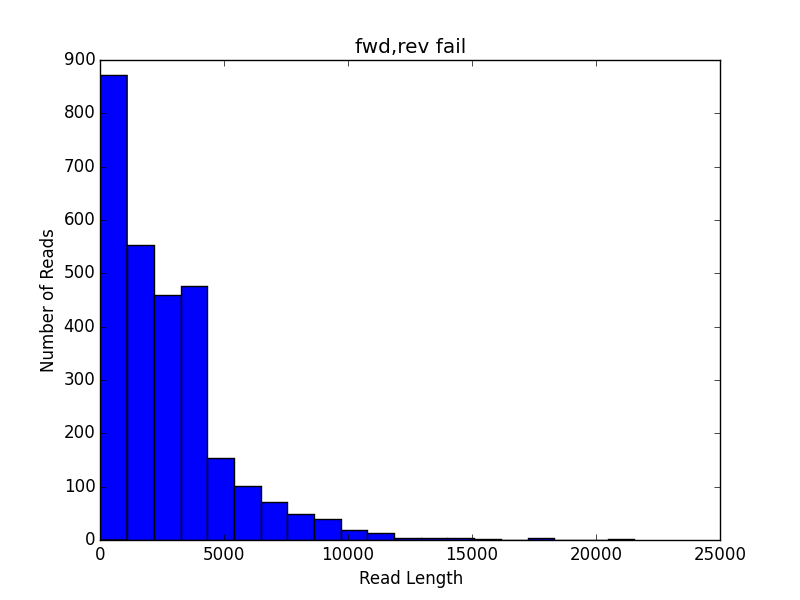
\includegraphics[width=.48\textwidth]{1Dfailures}
          \\
          Passed Reads
          &
          Failed Reads
        \end{tabular}
        

\subsection*{2D reads}

        The following histograms show the length distribution of 2D reads for passes and fails.

        
        \begin{tabular}{cc}
          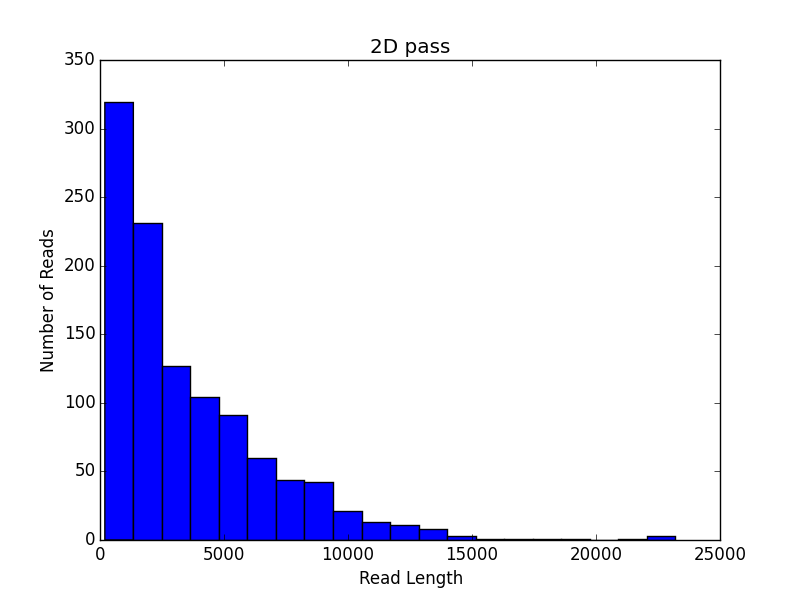
\includegraphics[width=.48\textwidth]{2Dpasses}
          &
          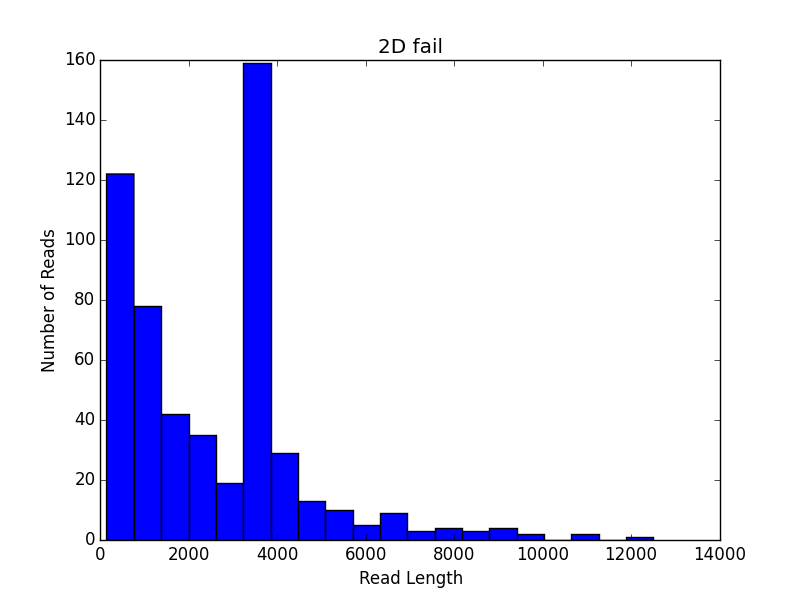
\includegraphics[width=.48\textwidth]{2Dfailures}
          \\
          Passed Reads
          &
          Failed Reads
        \end{tabular}

        
\subsection*{1D and 2D reads}

        The following histogramss show the cumulative length distribution of both 1D and 2D reads for passes and fails.

        
        \begin{tabular}{cc}
          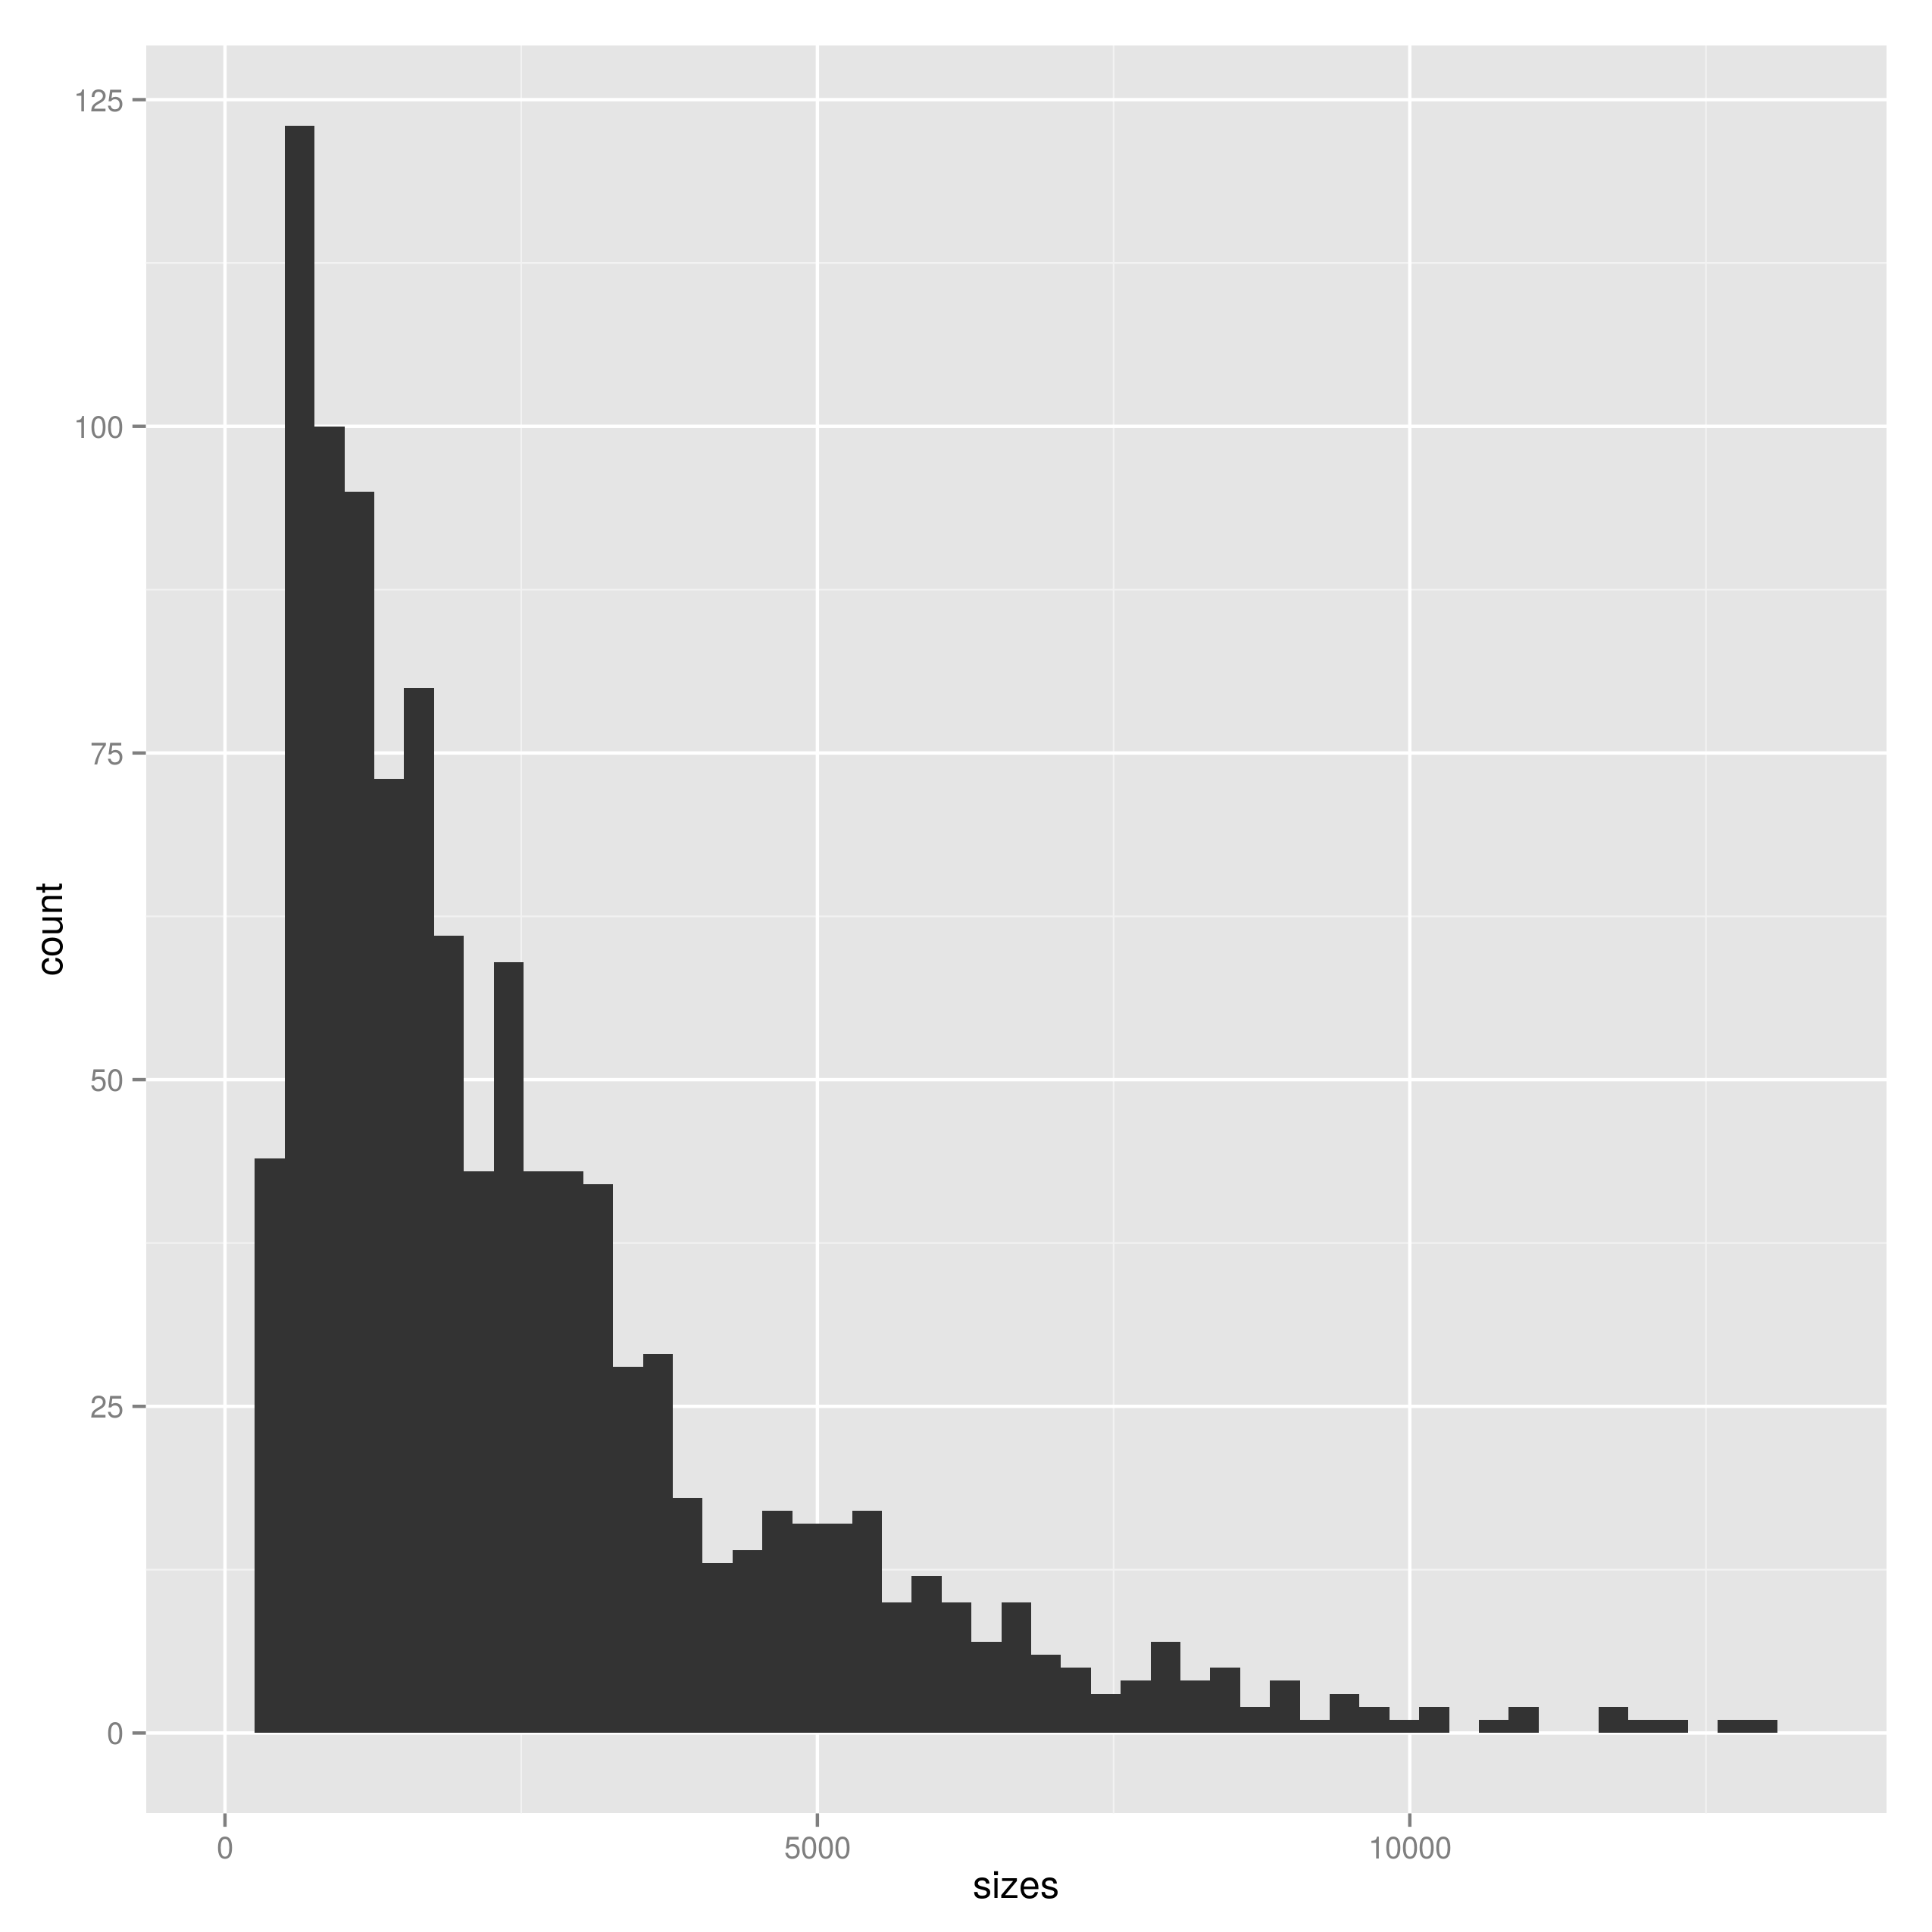
\includegraphics[width=.48\textwidth]{histallpass}
          &
          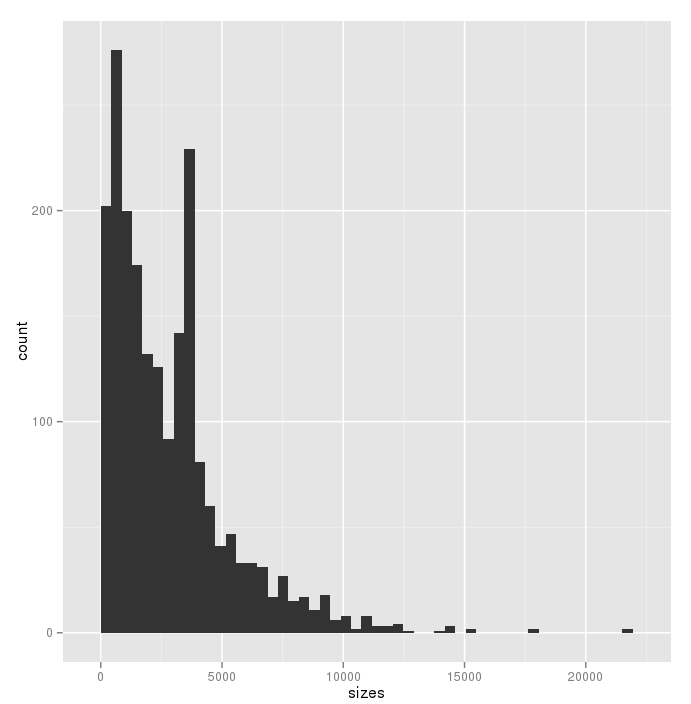
\includegraphics[width=.48\textwidth]{histallfail}
          \\
          Passed Reads
          &
          Failed Reads
        \end{tabular}
